\chapter{Soluzioni e tecnologie}
All'interno di questo capitolo andremo a definire una spiegazione generale delle tecnologie utilizzate all'interno della soluzione scelta per la gestione dei dati propria dei casi d'uso studiati. Ci soffermeremo inizialmente sulle nozioni che sono alla base, per poi andare a concentrarci sull'utilizzo specifico di un progetto open-source che rappresenta le fondamente dell'architettura presentata all'interno della soluzione, per poi concludere con la spiegazione dell'intera struttura funzionale.
\section{Cos'è una blockchain}
Una blockchain è un registro digitale aperto e distribuito, in grado di memorizzare record di dati (solitamente, denominati "transazioni") in modo sicuro, verificabile e permanente. Una volta scritti, i dati in un blocco non possono essere retroattivamente alterati senza che vengano modificati tutti i blocchi successivi ad esso e ciò, per la natura del protocollo e dello schema di validazione, necessiterebbe del consenso della maggioranza della rete. La blockchain è quindi rappresentabile come una lista, in continua crescita, di blocchi collegati tra loro e resi sicuri mediante l'uso della crittografia. Ad un blocco possono essere associate una o più transazioni e ogni blocco, inoltre, contiene un puntatore hash al blocco precedente e una marca temporale.
La natura distribuita e il modello cooperativo rendono robusto e sicuro il processo di validazione, ma presentano tempi non trascurabili, dovuti in gran parte al processo di validazione dei blocchi e alla sincronizzazione delle rete. L'autenticazione avviene tramite collaborazione di massa ed è alimentata da interessi collettivi. L'utilizzo di questa tecnologia consente anche di superare il problema dell'infinita riproducibilità di un bene digitale e della doppia spesa, senza l'utilizzo di un server centrale o di un'autorità.
Talvolta risulta possibile che alcuni nodi della rete producano simultaneamente più blocchi "concorrenti" (ossia collegati a uno stesso blocco già esistente, ma diversi tra loro nel contenuto): ciò dà origine a una biforcazione (fork) nella catena. Il protocollo di aggiornamento specifica quale regola i nodi debbano adottare per selezionare il blocco da accettare, tra quelli concorrenti. I blocchi non selezionati per l'inclusione nella catena sono chiamati blocchi orfani.
\section{Storia delle blockchain}
Mentre Bitcoin ha solo dieci anni, le origini della tecnologia blockchain sottostante ad esso, e ad altre migliaia di altre criptovalute, risalgono al 1991. Due scienziati hanno trovato un modo per utilizzare la crittografia per il timestamp di file digitali senza il rischio di manomissioni o retrodatazioni. Un anno dopo, è stato progettato un metodo efficiente per la raccolta di documenti in un blocco.
Questi metodi non avrebbero ottenuto un’applicazione significativa fino al 2004, quando lo scienziato informatico Hal Finney ha introdotto il concetto di proof-of-work token, che possono essere trasferiti da persona a persona. Questo concetto, ampiamente considerato come un primo prototipo di Bitcoin, risolse il problema della spesa doppia che esisteva in quel momento nelle soluzioni per le valute digitali.
Il 31 ottobre 2008 Satoshi Nakamoto ha introdotto un sistema di pagamento elettronico peer-to-peer decentralizzato chiamato Bitcoin. (Anche se fino ad ora, l’identità di Satoshi rimane un mistero). Il primo Bitcoin è stato quindi creato tramite mining, sempre da Satoshi, il 3 gennaio 2009. Satoshi ha quindi inviato 10 bitcoin a Hal il 12 gennaio 2009 — la prima transazione di Bitcoin al mondo.
Da lì sono emersi una manciata di progetti blockchain, uno dei quali ha portato alla creazione di varie criptovalute che fungono da alternative al Bitcoin. Nel 2013, il programmatore Vitalik Buterin ha iniziato a sviluppare Ethereum, una nuova piattaforma di calcolo distribuito basata sulla blockchain che consente la creazione di programmi o script, chiamati smart contract, nonché applicazioni decentralizzate. Una criptovaluta chiamata Ether viene utilizzata per pagare le transazioni sulla blockchain di Ethereum.
\newpage
\section{Distributed Ledger Tecnologies}
\begin{figure}[h]
    \centering
    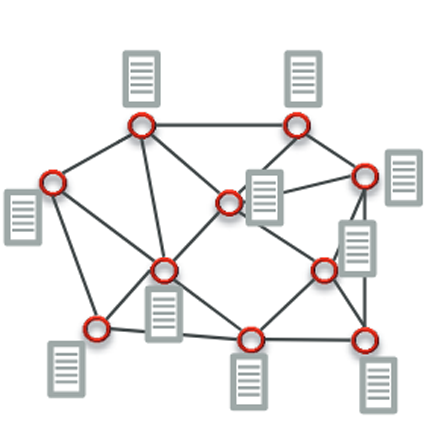
\includegraphics[width=0.5\textwidth]{img/dlt.png}
    \caption{Schema architettura di un distributed ledger}
    \label{fig:dlt}
\end{figure}

L'architettura di rete a cui fanno riferimento le blockchain moderne è basata su un Distributed Ledger. Tale architettura vede i vari nodi della rete collegati tra di loro secondo un'ottica basata sulla distribuzione di risorse, ossia su una decentralizzazione delle funzionalità di gestione dei dati basato su un archivio distribuito. Tale struttura non prevede nessuna organizzazione o entità di validazione dei dati centralizzati, questo aspetto garantisce sicurezza contro possibili alterazione di tale componente, garantendo cosi un livello di protezione implicito intrinseco proprio dell'architettura. Poichè non vi è nessuna validazione centralizzata, per poter definire se un dato sia corretto o meno, si ci avvale di un meccanismo di consenso che vede la partecipazione di più nodi attraverso un processo di votazione, che prevede la validazione o meno di una struttura dati. Le Distributed Ledger Tecnologies si basano proprio sulla gestione del meccanismo del consenso che, all'interno della logica di impostazione del registro decentralizzato,  archivia i dati contenuti all'interno della rete. L'adattabilità di tale logica all'interno del contesto su cui sono basate le blockchain, si ha con la validazione di un nuovo blocco da inserire all'interno della catena. Ogni blocco è formato da una o più transazioni che vengono effettuate all'interno della rete, se il blocco è valido per la maggior parte dei nodi della rete, esso è inserito all'interno della catena e diventa una struttura inalterabile. Il meccanismo del consenso delle DLT viene utilizzato dalla blockchain anche in caso di "forking" della catena, che prevedono il selezionamento di un blocco tra quelli proposti all'interno della rete e si avvalgono del sistema di validazione decentralizzato per poter selezionarne uno tra le possibili scelte ed inserirlo all'interno della catena. 
\section{Tipi di blockchain}
Dopo aver spiegato cos'è una blockchain, quali sono le componenti di base e come essa è strutturata, possiamo ora definire i vari tipi di blockchain che vengono utilizzate oggigiorno all'interno di vari progetti ICT. 
Le blockchain sono, essenzialmente, di tre tipi differenti: private, permissioned e public.
\subsection{Permissioned blockchain}
Le Blockchain permissioned sono soggette ad un’autorità centrale che determina chi possa accedervi. Oltre a definire chi è autorizzato a far parte della rete, tale autorità definisce quali sono i ruoli che un utente può ricoprire all’interno della stessa, definendo anche regole sulla visibilità dei dati registrati. Tali aspetti possono essere utili in molti casi d'uso; in cui si garantisce una gestione gerarchizzata o filtrata delle informazioni dei registri distribuiti, dove si possono definire dati che possono essere pubblici (visibili a tutti i nodi della rete) oppure privati (visibili solamente ad alcuni nodi, quest'ultimo tipo di dati può essere filtrato e reso visibile solamente da una categoria di nodi aventi particolari caratteristiche). Le Blockchain permissioned introducono, quindi, il concetto di centralizzazione della gestione dei dati su un'architettura basata, però, su aspetti come la decentralizzazione e la distribuzione erecditate dalle architetture DLT su cui si basano le blockchain. Quest'ultima caratteristica è molto utile per ridurre i costi di validazione. Infine, il meccanismo del consenso interessa solo un sottoinsieme di nodi e non tutti quelli della rete, la selezione di quali nodi abbiano il diritto di partecipazione al consenso è collegata ai criteri interni alla blockchain. 
\subsection{Private blockchain}
\begin{figure}[h]
    \centering
    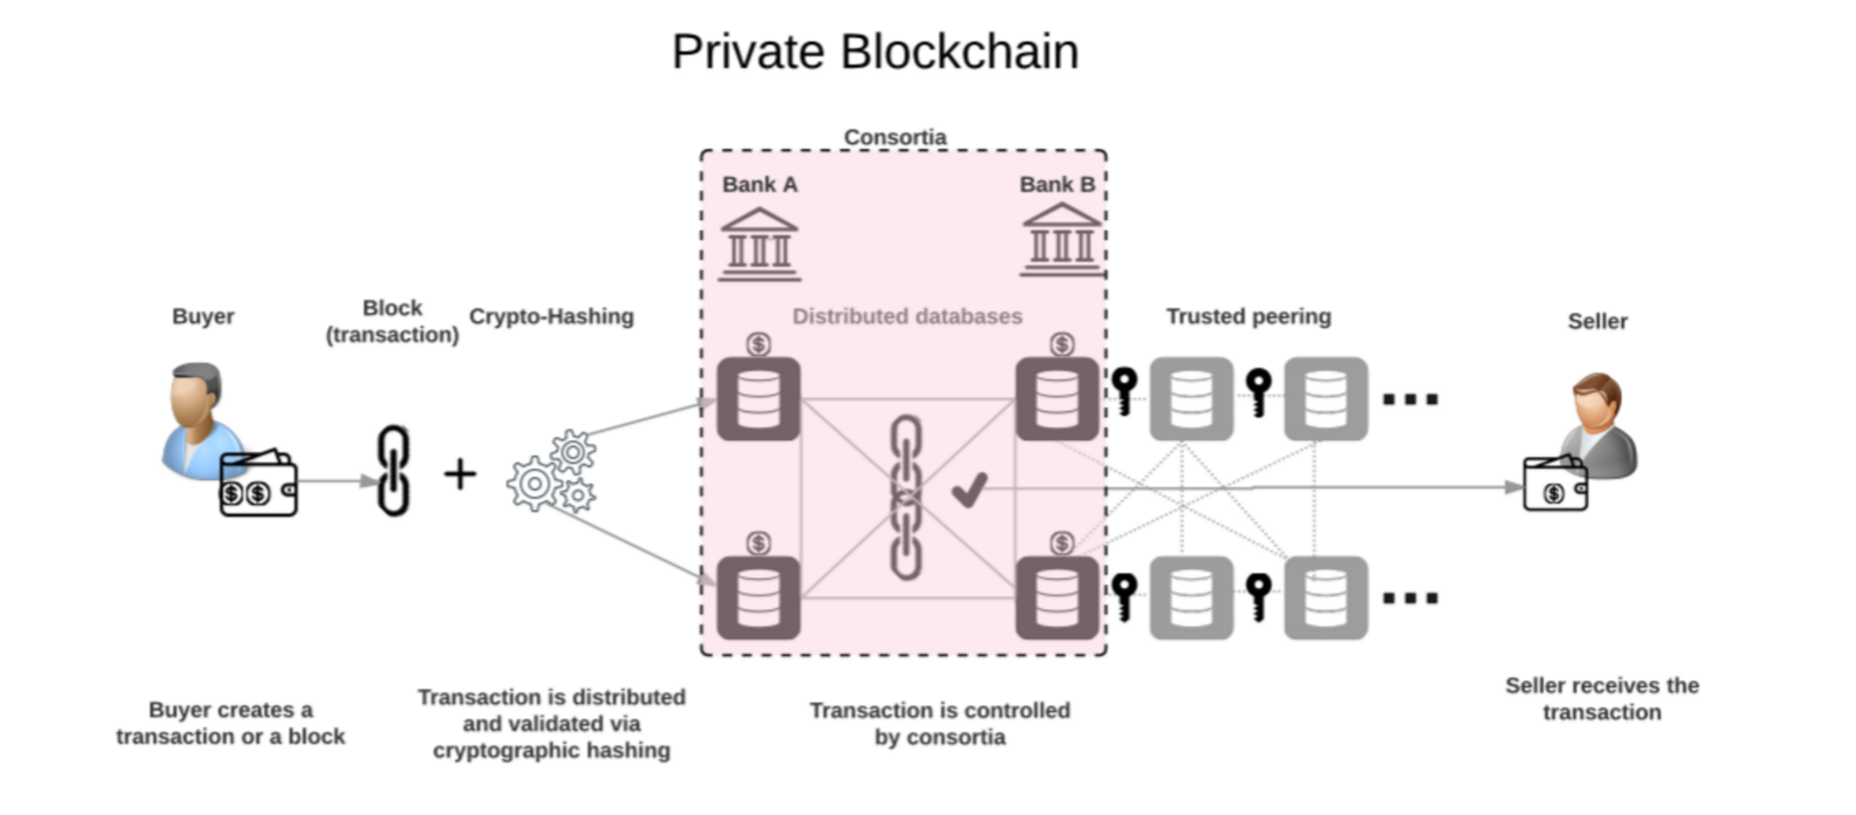
\includegraphics[width=1\textwidth]{img/private-blockchain.png}
    \caption{Caso d'uso di una transazioni in una private blockchain}
    \label{fig:private-blockchain}
\end{figure}
Le blockchain private condividono alcune caratteristiche con le blockchain permissioned. Questo tipo di blockchain viene controllata da una organizzazione centrale che ha la funzione di gestire gli accessi in rete da parte dei vari nodi che tentano di inserirsi. Tale organizzazione è formata da nodi affidabili che vengono ritenuti sicuri e attendibili. Questa organizzazione è alla base non solo della gestione degli accessi, ma anche della manipolazione delle regole di amministrazione dei dati. Quindi, vediamo che tale organizzazione ha la possibilità di variare le regole di gestione delle informazioni contenute nei nuovi blocchi che vogliono aggiungersi alla catena; ossia possono manipolare liberamente le regole di validazione delle transazioni effettuate dai nodi della blockchain
\subsection{Public blockchain}
\begin{figure}[h]
    \centering
    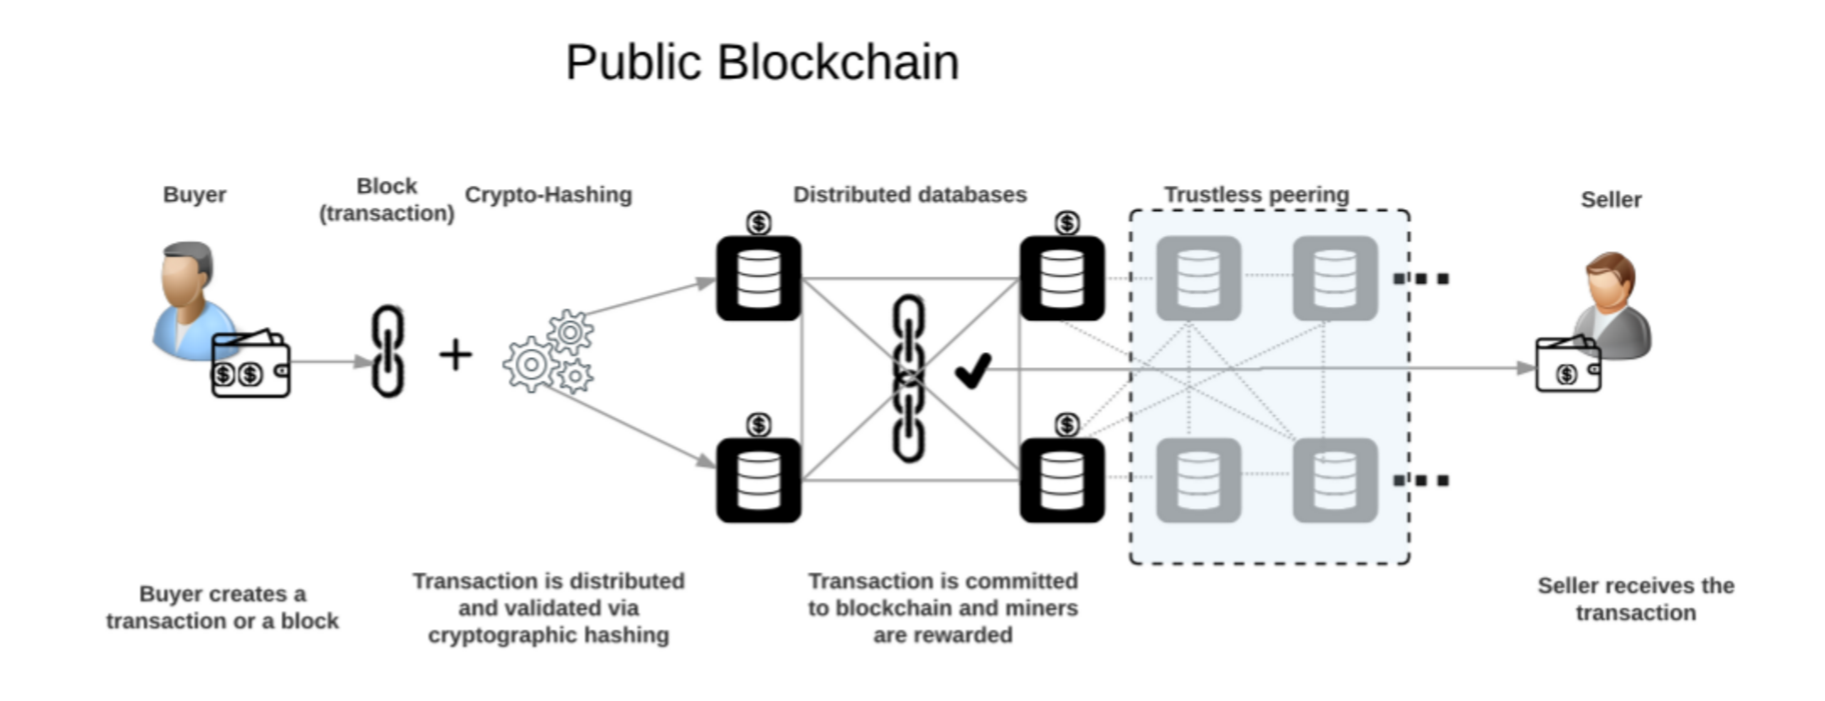
\includegraphics[width=1\textwidth]{img/public-blockchain.png}
    \caption{Caso d'uso di una transazioni in una public blockchain}
    \label{fig:public-blockchain}
\end{figure}
Le public o permissionless blockchain sono essenzialmente il modello principale che raffigura una rete accessibile da chiunque, senza nessuna forma di autorizzazione o autenticazione. Ogni nodo della rete può ricevere o mandare delle transazioni. Ogni nodo è messo allo stesso livello di tutti gli altri della rete, andando a rispettare la natura distribuita della DLT su cui si basano le blockchain. Quando si genera una transazione o si genera un blocco, esso viene sottoposto alla validazione decentralizzata basata sul meccanismo di consenso. Quindi, vediamo che i nodi della rete hanno principalmente due ruoli fondamentali: Il primo è quello di generare o ricevere le transazioni da o verso la blockchain, il secondo è quello di partecipare al meccanismo di validazione delle varie transazioni che andranno ad essere inserite all'interno dei blocchi che andranno a costituire la catena. 
\section{Procedimento di creazione di un blocco}
Come spiegato precedentemente, quando si effettuano delle operazioni su dati all'interno dell'archivio distribuito mantenuto nella blockchain, si ha una transazione. Dopo la sua creazione, una transazione viene inserita in un blocco che deve essere validato da una serie di nodi denominati miner. I miner sono quei nodi che sono adibiti alla verifica di un blocco. Il processo di validazione di un blocco si concentra su un'operazione di ricerca di un valore che, se aggiunto ad altre informazioni del blocco sotto analisi, restituisca un determinato codice hash. La ricerca di tale valore è concorrente tra i vari miner interessati nel processo di verifica che competono per ritrovare tale valore corretto. Quando uno dei vari miner riesce a trovare il valore richiesto, si passa ad una fase di verifica da parte di tutti gli altri miner per certificare la correttezza del risultato. In caso affermativo, il miner che ha trovato il risultato desiderato riceve, in genere, un token. Tale token può essere una moneta virtuale come i Bitcoin. Il processo di verifica della correttezza del valore da parte di tutti gli altri miner interessati nella validazione viene definito come proof-of-work o PoW. In seguito, il blocco verificato viene aggiunto alla catena che identifica la blockchain aumentando cosi la sua lunghezza.
\newpage
\subsection{Funzione di Hash}
\begin{figure}[h]
    \centering
    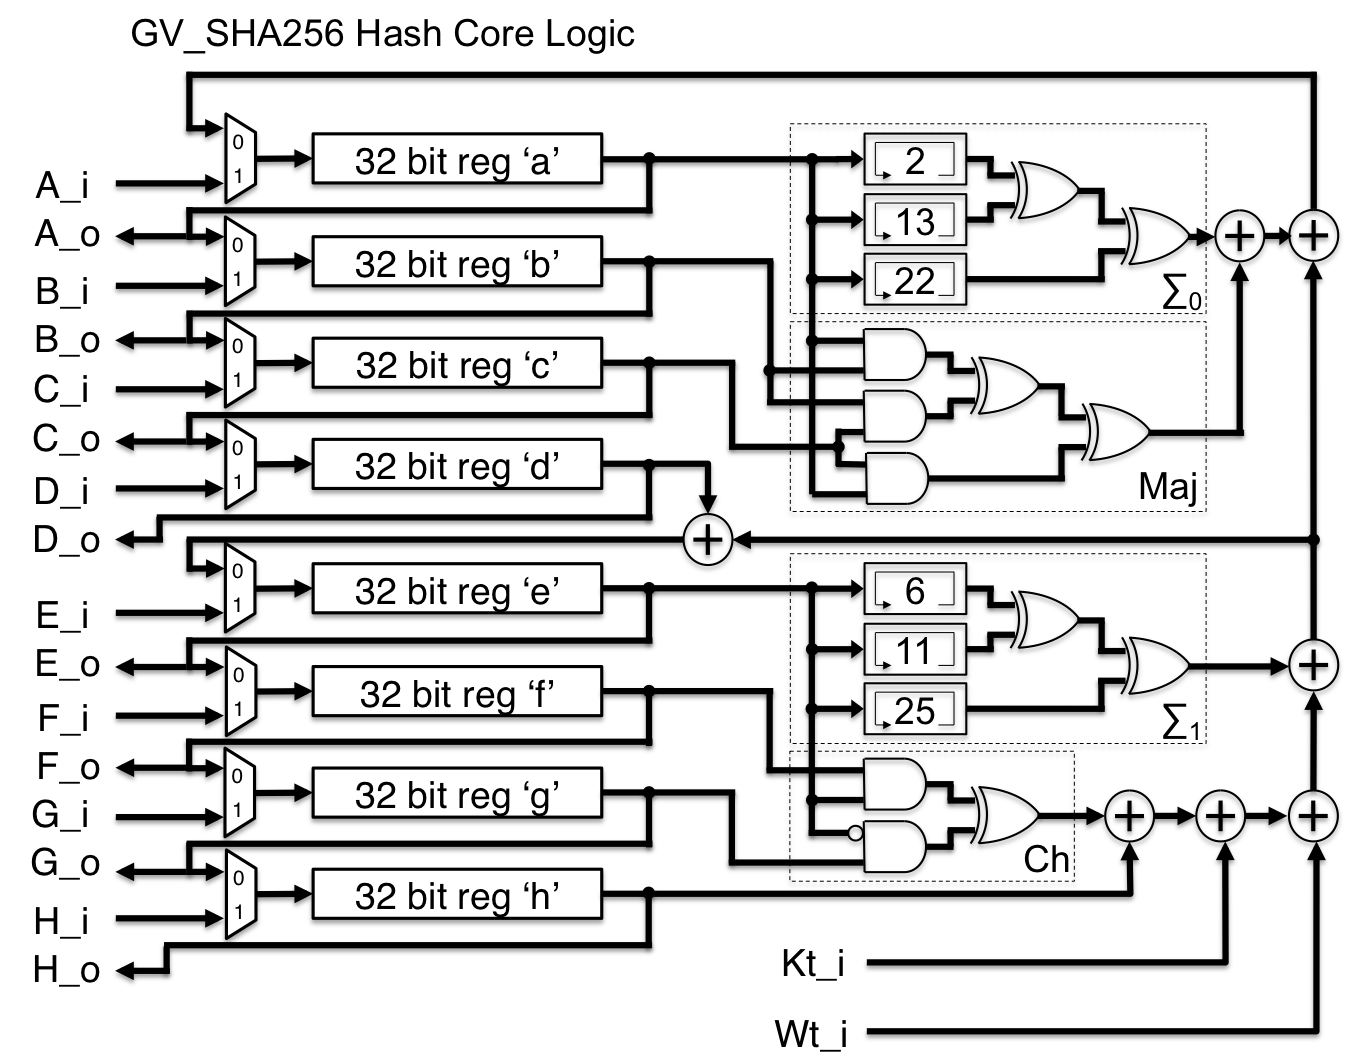
\includegraphics[width=0.78\textwidth]{img/sha256.png}
    \caption{Logica Hash Code SHA-256}
    \label{fig:sha256}
\end{figure}
La ricerca del valore e la generazione di un codice hash viene definito secondo un particolare algoritmo di crittografia. All'interno delle blockchain moderne, secondo una visione ad alto livello, l'algoritmo di hash prende in input una serie di dati che possono essere di lunghezza variabile e, tramite una funzione di hash, si ha la conversione ad una stringa di caratteri di lunghezza predefinita raffigurante l'output della funzione. Tale procedimento è irriversibile, nel senso che non è possibile risalire alla stringa di input partendo da quella di output. Generalmente, la funzione di hash che si utilizza all'interno di una blockchain è lo SHA-256, esso usa una funzione che restituisce sempre una stringa di lunghezza fissa pari a 256 bit. Il procedimento di ricerca prevede di applicare una serie di operazioni in cui si specificano una successione di tentativi di input, una conversione di quest'ultimo alla stringa hash corrispondente e una verifica andando a confrontarla con la stringa codificata da decifrare. Se la codifica dell'input e la stringa ricercata combaciano, allora si è trovato il valore ricercato. Notiamo che dato uno specifico input, si avrà sempre un medesimo output ad ogni conversione effettuata. La difficoltà nel trovare una possibile stringa di input partendo dalla stringa di output è alla base della gestione dello SHA-256. Questo perchè vi sono al più una possibile combinazione che potrebbero corrispondere alla stringa di input ricercata. Inoltre, vediamo che non vi è nessun criterio ancora conosciuto su come tale funzione hash possa essere prevista se non tramite algoritmi di risoluzione basati sulla brute-force. Lo SHA-256 è alla base della crittografia moderna, andando ad essere applicato su qualsiasi forma di sicurezza e mascheramento di dati all'interno dell'ambito ICT. 
\section{Applicazione della funzione Hash}
Più nello specifico, nell'applicazione della funzione hash, si ha che i miner di una blockchain sfruttano il loro poter computazionale per trovare un numero (chiamato nonce). Questo, se processato tramite la funzione di hash, insieme ad altri dati presenti nel blocco da validare, deve restituire un risultato codificato che inizia con un determinato numero di zeri. Questo codice viene chiamato "hash della testa del blocco". Il numero di zeri richiesti definisce il grado di difficoltà per la validazione del blocco, in quanto maggiore è il numero di zeri e maggiore è la difficoltà di validazione (il numero di zeri richiesti è definito in uno dei dati presenti nel blocco). Quindi lo scopo principale per la validazione di un blocco è quella di trovare un nonce in modo tale che, aggiunto agli altri dati del blocco ci dia come risultato la stringa hash in SHA-256 corrispondente. Non esiste una tecnica o un calcolo per trovare un nonce valido, l'unico modo logico per farlo è tramite numerosi tentativi casuali. Proprio per questo motivo, i miner si servono di appositi hardware che misurano la loro potenza in "tentativi al secondo" (H/s). Da qui nasce il concetto di "competizione tra miner", in quanto solo il miner che troverà per primo un nonce valido verrà ricompensato per il lavoro svolto. Prima di essere ricompensato però, il miner che trova un nonce valido comunica la soluzione agli altri nodi della rete, questi effettueranno una verifica per confermare che il nonce sia valido. Qualora il nonce non fosse valido, la competizione si riapre e tutti i miner tornano alla ricerca del medesimo nonce.
\newpage
\section{Crittografia asimmetrica e gestione delle criptovalute}
La crittografia asimmetrica si basa sull'utilizzo di una coppia di chiavi: Una pubblica e una privata. La chiave pubblica è visibile a tutti i nodi di una rete, che possono sfruttarla per criptare un dato all'interno di una trasmissione, la chiave privata è propria di ogni nodo, quindi non è condivisa con gli altri dispositivi della rete; essa serve per decriptare un messaggio o un dato trasmesso all'interno del network. Quando un messaggio viene criptato tramite una chiave pubblica, esso potrà successivamente essere decriptato solamente dal possessore della chiave privata corrispondente. Tale aspetto, fa si che qualsiasi dispositivo possa criptare il nodo e solamente quello proprietario possa decriptarlo. Facciamo un esempio per chiarire quanto appena detto. Abbiamo due persone: A e B. A vuole inviare un documento di testo a B, ma vuole accertarsi del fatto che solo B sia in grado di leggere il contenuto di tale documento. A decide allora di utilizzare la crittografia asimmetrica, si serve quindi della chiave pubblica di B per criptare il suo messaggio (A conosce la chiave pubblica di B in quanto, essendo appunto pubblica, B l'ha messa a disposizione di A). Il documento così criptato non è più decifrabile da A, in quanto non è in possesso della chiave privata di B (questa, al contrario della chiave pubblica, è appunto privata: solo B ne è in possesso). B riceve il documento e riesce a decifrarlo utilizzando la sua chiave privata. 


\begin{figure}[h]
    \centering
    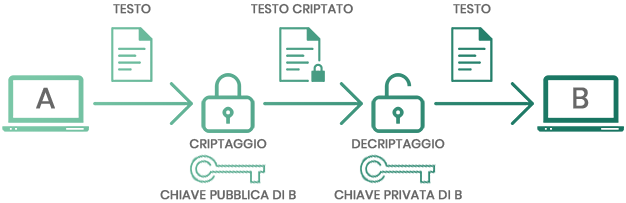
\includegraphics[width=0.78\textwidth]{img/asymmetric-cripto.png}
    \caption{Simulazione di crittografia asimmetrica}
    \label{fig:asimmetric-crypto}
\end{figure}
Vediamo ora come tale procedura viene utilizzata all'interno di una blockchain. La crittografia asimmetrica viene utilizzata all'interno della gestione di una transazione che vede il trasferimento tra due account di una criptovaluta o di dati da o verso un'account. Notiamo che una delle principali caratteristiche che si hanno sulla transazione è come essa viene trasferita. Secondo uno schema standard, si distingue l'account mandante da quello ricevente. All'interno della transazione si fa uso della chiave privata e pubblica del ricevente. Quando si effettua una transazione, il mandante cripta utilizzando la chiave pubblica del ricevente, tale procedimento è possibile poichè la chiave è all'interno delle informazioni note del mandante. In seguito, la transazione può essere decriptata solamente dal ricevente, questo perchè se si effettua un'operazione di criptaggio utilizzando una chiave pubblica, essa può essere decriptata solamente dalla rispettiva chiave privata che, come detto precedentemente, è propria solamente dell'account possessore che, in questo caso, è l'account ricevente. Quando si ha una transazione incentrata sul trasferimento di una criptovaluta, il procedimento sussiste anche nell'estrazione e nel deposito sui wallet degli account interessati. I wallet sono dei "portafogli virtuali" che mantengono solamente traccia della transazione mentre le criptovalute sono mantenute all'interno del ledger su cui si fonda la blockchain.

\section{Proof-of-Work}
Il concetto originale di Proof-of-Work risale al 1993, anno in cui è stato sviluppato per prevenire attacchi denial of service e altre violazioni come network spam. Sostanzialmente questa soluzione richiedeva un po’ di lavoro all’utente del servizio, inteso come tempo di lavorazione di un computer.
Nel 2009, Bitcoin ha introdotto un metodo innovativo per utilizzare la Proof-of-Work come algoritmo di consenso per convalidare transazioni e trasmettere nuovi blocchi alla blockchain. 
Da allora si è diffuso fino a diventare un algoritmo di consenso ampiamente utilizzato nelle blockchain. Il Proof-Of-Work si basa su due operazioni fondamentali:
\begin{enumerate}
    \item Risoluzione di enigmi computazionali: Difficile da ottenere, si sfrutta il potere computazionale per trovare il valore corrispondente ad una stringa hash. Dato che la funzione di hash è irreversibile, la ricerca della soluzione ha una complessità computazionale basata su una ricerca in brute-force.
    \item Verifica della soluzione: Facile da ottenere, non si fa altro che applicare sul valore risultato la funzione di hash e verificare che l'output sia quello corretto.
\end{enumerate}
In sintesi, i miner all’interno di una rete competono tra di loro per risolvere enigmi computazionali complessi. E’ difficile trovare la soluzione di questi enigmi, ma allo stesso tempo è facile verificare se questa è corretta. Quando un miner trova la soluzione a un'enigma, può trasmettere il blocco alla rete, e tutti gli altri miner verificano che la soluzione sia effettivamente corretta.
\section{Proof-of-Stake}
L’algoritmo Proof-Of-Stake utilizza un processo di elezione pseudo-casuale per selezionare un nodo che agirà da validatore univoco del blocco successivo, in base a una combinazione di fattori che possono includere periodo di staking, randomizzazione e fondi di proprietà del nodo. L'algoritmo di selezionamento del nodo è variabile e definisce varie forme che, sotto un punto di vista procedurale, varia solamente per l'aspetto di selezionamento.
\subsection{Forging}
E’ bene osservare che, nei sistemi Proof-of-Stake, l’inserimento di nuovi blocchi nella blockchain viene chiamato con il termine di forging invece che di mining, quindi i blocchi vengono 'forgiati'. Una buona parte delle criptovalute che utilizzano la Proof-of-Stake iniziano vendendo monete pre-minate, oppure sfruttano l’algoritmo Proof-of-Work e in seguito passano alla Proof-of-Stake.
Mentre nei sistemi basati sulla Proof-of-Work viene creata nuova moneta per ricompensare i miner, generalmente il sistema Proof-of-Stake distribuisce come premio solo le commissioni sulle transazioni.
Gli utenti che vogliono partecipare al processo di forging devono congelare una certa somma di monete all’interno del network, mettendo quindi un’adeguata posta in gioco. Le dimensioni della stake, ossia le criptovalute messe in gioco, determinano le probabilità di un nodo di venir selezionato come validatore e agire da forger del blocco successivo - più grande la stake, maggiori le probabilità. Tuttavia, per fare in modo che questo processo non favorisca solo i nodi più ricchi del network, il processo di selezione presenta altri metodi unici. I più comuni sono ‘Randomised Block Selection’ e ‘Coin Age Selection’.
\newpage
\subsection{Randomised Block Selection}
Con il metodo Randomised Block Selection, i validatori vengono selezionati cercando i nodi con una combinazione tra valore hash più basso e stake più grande. Dato che le dimensioni delle stake sono pubbliche, in genere gli altri nodi possono prevedere quale verrà selezionato.
\subsection{Coin Age Selection}
Il metodo Coin Age Selection sceglie nodi in base a quanto tempo hanno lasciato i propri token congelati come stake. La coin age viene calcolata moltiplicando il numero di giorni per il numero di monete congelate. Quando un nodo forgia un blocco, la sua coin age viene resettata a zero e deve aspettare un certo periodo di tempo prima di poter essere selezionato - questo impedisce ai nodi con grandi stake di dominare la blockchain.
\subsection{Inserimento di un blocco tramite Proof of Stake}
Ogni criptovaluta che usa l’algoritmo Proof of Stake presenta una propria lista di regole e metodi per creare la migliore combinazione possibile per il network e per gli utenti.
Quando un nodo viene selezionato come forger del blocco successivo, deve controllare se le transazioni in esso contenute sono valide, firmare il blocco e aggiungerlo alla blockchain. Come ricompensa, il nodo riceve le commissioni associate alle transazioni nel blocco.
Se un nodo vuole smettere di partecipare al processo di forging, deve attendere un certo periodo di tempo prima di poter accedere alla propria stake e alle ricompense guadagnate, lasciando al network tempo per verificare che non abbia aggiunto blocchi fraudolenti alla blockchain. La stake funge da incentivo economico che dissuade il nodo forger dal convalidare o creare transazioni fraudolenti. Se il network individua una transazione fraudolenta, il nodo forger perde parte della sua stake, oltre al diritto a partecipare come forger in futuro. Quindi, a patto che la stake sia più grande della ricompensa, il validatore che tenta di raggirare il sistema perderebbe molto di più rispetto a quello che riuscirebbe a guadagnare. Per riuscire a raggiungere un controllo effettivo del network e approvare transazioni fraudolente, un nodo dovrebbe possedere una stake maggioritaria, situazione conosciuta come 51\% attack. A seconda del valore di una criptovaluta, un attacco del genere risulta quasi irrealizzabile dato che per ottenere il controllo del network sarebbe necessario acquisire il 51\% delle unità in circolazione.I vantaggi principali dell’algoritmo Proof of Stake sono l’efficienza energetica e la sicurezza. La facilità e l’accessibilità incoraggia un maggior numero di utenti a impostare e mantenere nodi. Questo, insieme al processo di randomizzazione, rende il network più decentralizzato, in quanto non sono più necessarie mining pool per aggiungere blocchi. Inoltre, dato che non vengono più distribuite nuove monete come ricompensa, il prezzo di una particolare moneta rimane più stabile.
\subsection{Utilità del Proof-of-Stake}
In conclusione, una delle caratteristiche principali che delineano l'utilizzo del Proof-of-Stake rispetto al meccanismo delineato dal Proof-of-Work è che nel primo caso si ha una utilità di natura transazionale, il forger scelto non fa altro che delineare una ricompensa solamente per essere stato selezionato nella convalida di un blocco senza creare la criptovaluta guadagnata ma utilizzarne una pre-minata, ciò ha come vantaggio non solo quello di definire un meccanismo di premiazione ben concisa, ma riesce anche ad evitare lo sforzo computazionale che si aveva nel Proof-of-Work.
\newpage
\section{Smart Contract}
Uno smart contract è un vero e proprio contratto in codice, scritto su una blockchain. Questo viene utilizzato per regolamentare una transazione tra due o più parti. Questo contratto viene definito intelligente (smart), in quanto è in grado di verificare se determinate condizioni, definite alla base (nel codice) del contratto stesso, sono avvenute ed è in grado di eseguirsi automaticamente - portando a termine la transazione tra le parti - nel momento in cui tali condizioni sono state raggiunte e/o verificate.
La funzione alla base di uno smart contract è in grado di leggere sia le condizioni che le clausule concordate nel contratto: non appena i dati riferiti a situazioni reali corrispondono alle condizioni e ai dati riferiti nelle clausule concordate, il contratto intelligente viene eseguito, portando a termine la transazione tra le parti.
Nella stesura e creazione di uno smart contract bisogna essere estremamente precisi. Le parti che sottoscrivono il contratto devono scegliere con cura le condizioni, le clausule e le fonti di dati su cui il contratto è chiamato ad attenersi. Lo smart contract è quindi un programma che elabora, in maniera deterministica, le informazioni che vengono raccolte, in questo modo si ha la certezza di un giudizio oggettivo, escludendo inevitabilmente qualsiasi forma di interpretazione.
\begin{figure}[h]
    \centering
    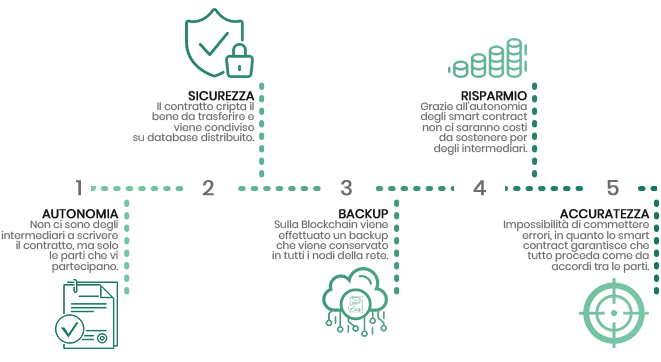
\includegraphics[width=0.9\textwidth]{img/smart-contract.png}
    \caption{Vantaggi derivati dall'uso di uno smart contract}
    \label{fig:smart-contract}
\end{figure}
Grazie agli smart contract è finalmente possibile eliminare qualsiasi tipo di intermediario e i costi a essi associati, in quanto non potrà mai esistere qualcosa o qualcuno che sia più preciso e affidabile di uno smart contract.
Ai contraenti spetta il compito di definire le condizioni, le clausole, le modalità, le regole di controllo e di azione, ma una volta che il contratto è stato scritto e accettato, i contraenti non potranno in alcun modo modificare o annullare la transazione. Gli effetti della transazione non dipendono più dalla volontà dei contraenti, in quanto sarà il contratto a portare a termine il tutto senza soggettività, così come è stato definito nel contratto in maniera completamente sicura e trasparente.
\section{Forking}
Una delle caratteristiche che raffigurano un software generico è la necessità di aggiornamenti. Tali aggiornamenti possono rappresentare delle modifiche da apportare all'interno delle regole di gestione dei dati come cambiamenti sulle regole di validazione di un blocco all'interno delle blockchain, la sua dimensione, le modalità di gestione delle ricompense o la tipologia di cryptovaluta utilizzata. In generale, quando si parla di regole si fa sempre riferimento ad un protocollo che, nel contesto delle blockchain, si riferiscono alla gestione dei blocchi e dei dati all'interno dei vari nodi della rete. La gestione degli aggiornamenti all'interno di una blockchain viene definito con il termine di forking. Esistono due tipologie di forking: Soft fork e Hard fork, in entrambi i casi vi è una modifica del protocollo, la differenza sostanziale si vede nella convalida dei blocchi e come vengono gestiti i consensi o le negazione da parte dei nodi aggiornati al nuovo protocollo e quelli ancora con la versione precedente.
\subsection{Soft fork}
Le soft fork sono delle modifiche retro-compatibili, ossia delle modifiche in cui la versione aggiornata e quella precedente hanno nella loro definizione delle caratteristiche non contrastanti. Tale aspetto ha come risultato quello di poter far elaborare nuove transazioni e aggiungere nuovi blocchi alla catena da parte dei nodi che ancora non hanno subito l'aggiornamento del protocollo se le proprietà dei nuovi blocchi rispettano le regole della nuova versione.
\begin{figure}[h]
    \centering
    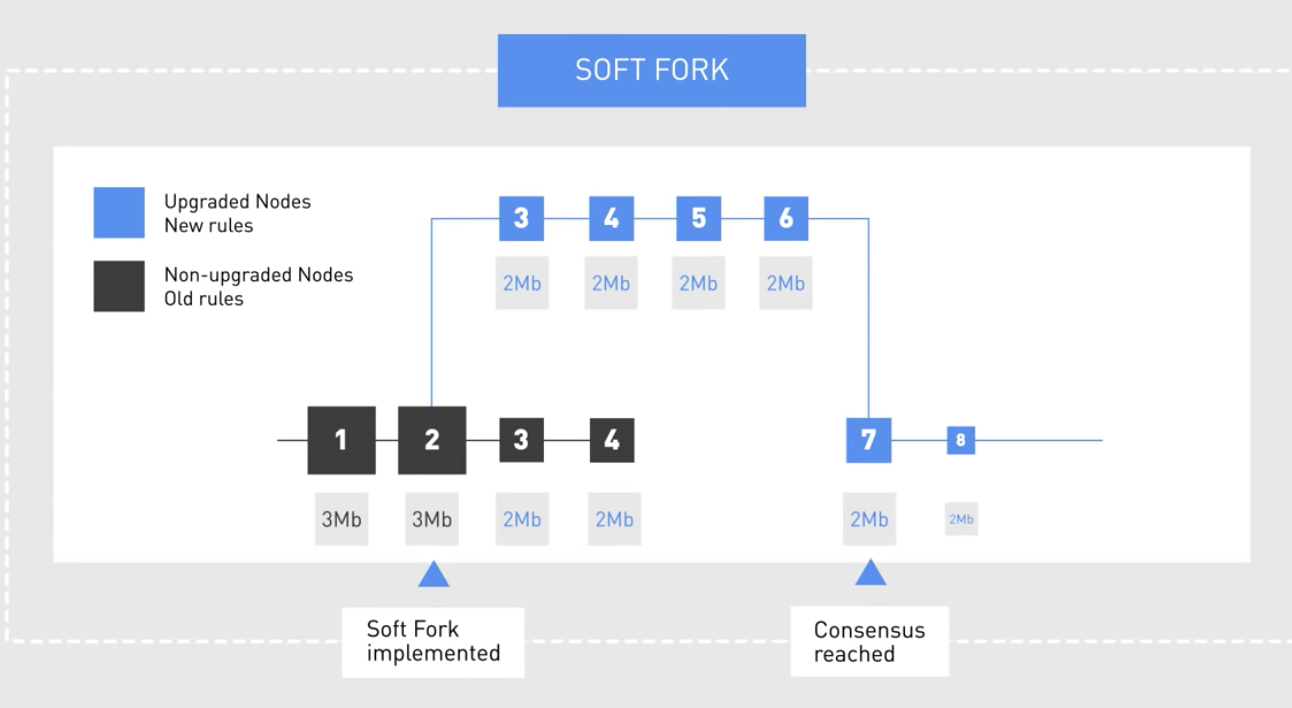
\includegraphics[width=0.8\textwidth]{img/soft-fork.png}
    \caption{Procedura di soft fork}
    \label{fig:soft-fork}
\end{figure}
Un esempio di soft fork si può avere nella modifica del protocollo sulla grandezza del blocco da aggiungere alla catena. Se si ha una riduzione della dimensione da 3 MB a 2 MB e i nodi non aggiornati producono un blocco con dimensione pari o non superiori a 2 MB, essi vengono comunque validati da parte dei nodi aggiornati poichè rispettano ugualmente le proprietà delle nuove regole del protocollo. Se invece producono un blocco superiore a 2 MB, esso verrà rifiutato poichè non conforme secondo le regole dei nodi aggiornati.
\subsection{Hard fork}
Sono delle modifiche che creano delle biforcazioni contrastanti tra di loro poichè l'aggiornamento del protocollo rende incompatibile la versione antecedente rispetto quella attuale, causando l'impossibilità di generare dei nuovi blocchi da parte dei nodi ancora non aventi la versione corrente del protocollo sotto analisi. In genere un hard fork si presenta quando si intende aggiornare ed estendere un protocollo già esistente oppure quando si vuole definire una catena di blocchi indipendente rispetto a quella della versione precedente. 
Immaginando una modifica in un protocollo che aumenta la dimensione dei blocchi da 2 MB a 4 MB. Se un nodo aggiornato prova ad aggiungere un blocco pari a 3 MB nella blockchain, i nodi non aggiornati vedranno tale blocco come non valido, andandolo a rifiutare.
Gli hard fork hanno due forme specifiche:
\begin{enumerate}
    \item Hard fork programmati
    \item Hard fork controversi
\end{enumerate}
\begin{figure}[h]
    \centering
    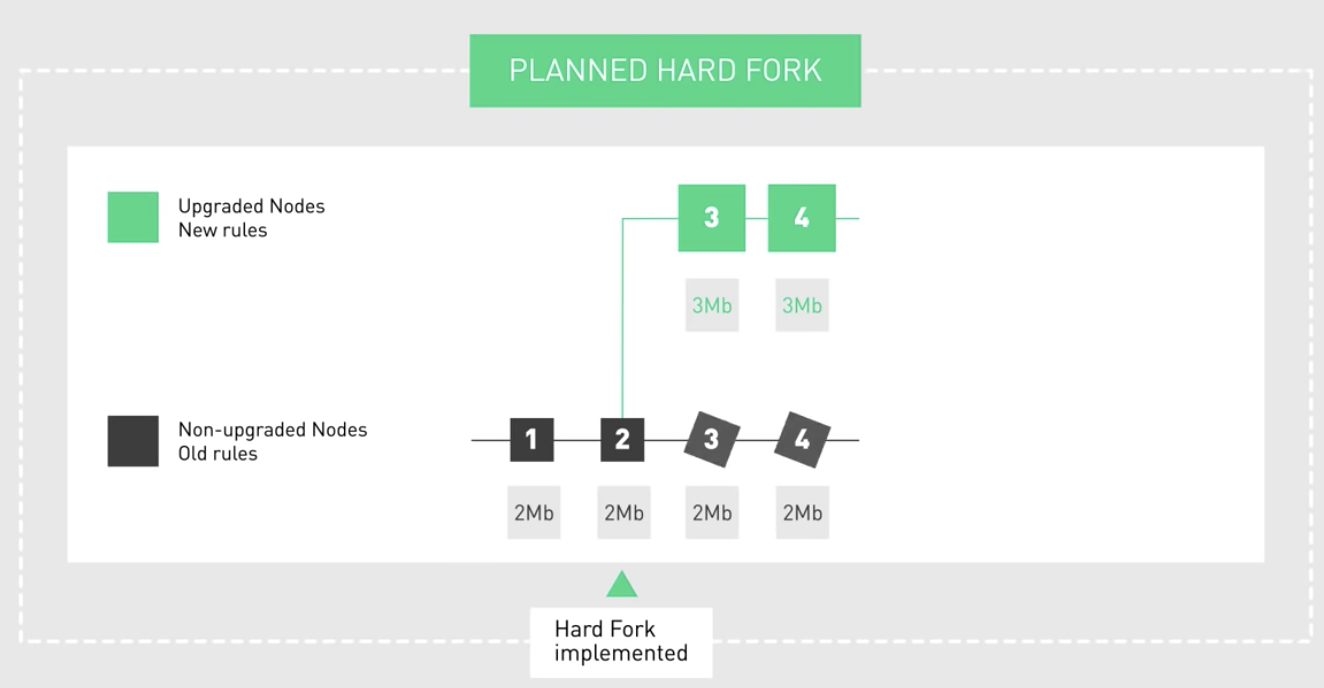
\includegraphics[width=0.8\textwidth]{img/planned-fork.png}
    \caption{Schema di Hard Fork Programmato}
    \label{fig:planned-fork}
\end{figure}
Nel primo caso, i nodi aggiorneranno automaticamente il protocollo, ignorando la vecchia versione. In questo caso, si avrà un forking in cui vede la differenza nel consenso tra i nodi aggiornati e quelli non aggiornati che continueranno ad operare sulla vecchia catena finchè non verranno aggiornati, andando, così, ad abbandonarla definitivamente. Tale forma di hard fork viene effettuata quando tutti i nodi sono d'accordo sulle modifiche da effettuare e, quindi, vi è un'aggiornamento di massa senza nessuna divisione decisoria. 
\begin{figure}[h]
    \centering
    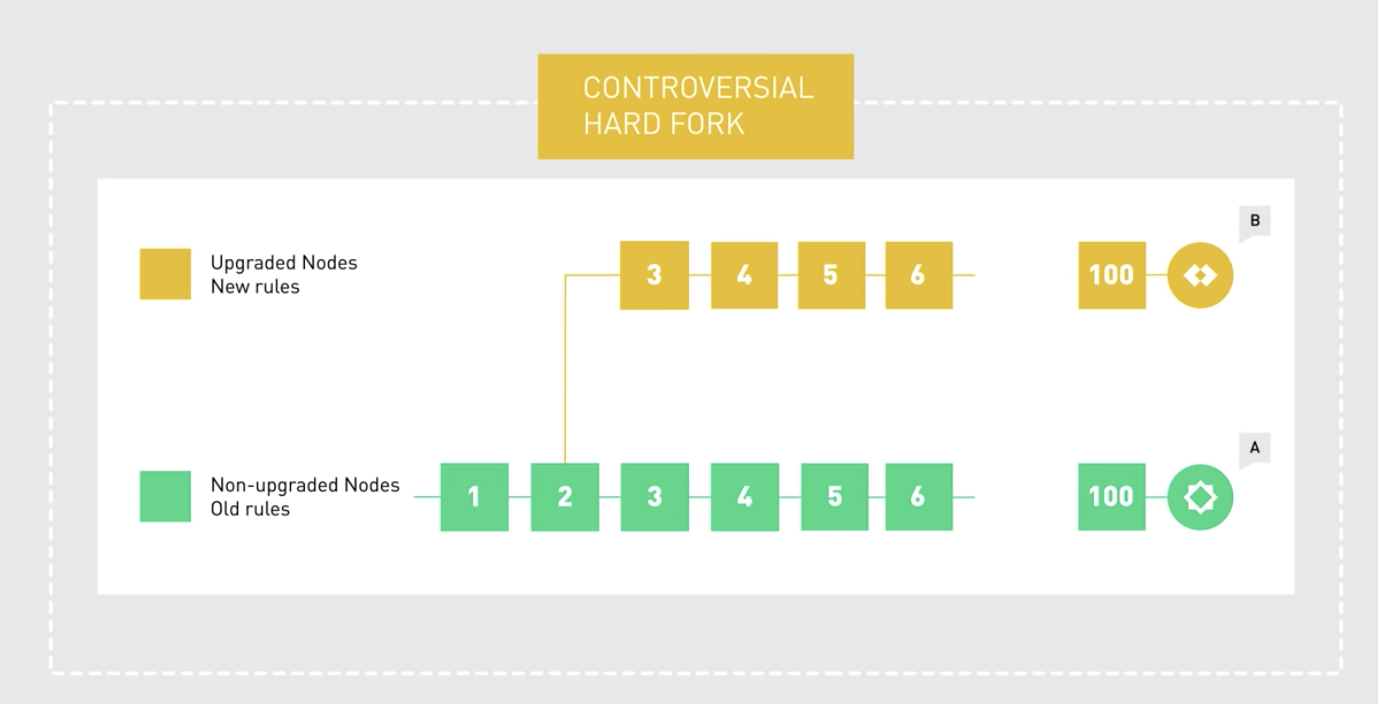
\includegraphics[width=0.8\textwidth]{img/controversial-fork.png}
    \caption{Schema di Hard Fork Controverso}
    \label{fig:controversial-fork}
\end{figure}
Nel secondo caso, la biforcazione si effettua anche sotto un punto di vista di scelta nell'aggiornare o meno il protocollo della blockchain. Con gli hard fork controversi si ha come risultato finale la creazione di due blockchain separate, indipendenti ed incompatibili. Ogni blockchain avrà una propria criptovaluta, i nodi che parteciperanno ad una delle due biforcazioni si distingueranno a secondo dell'aggiornamento o meno del protocollo. 
Dato che un fork si basa sulla blockchain originale, tutte le transazioni che sono state effettuate andranno ad essere copiate nella nuova blockchain. Per esempio, se possiedi 100 monete di una criptovaluta chiamata Moneta A, e un hard fork basato su tale criptovaluta ne crea una nuova chiamata Moneta B, riceverai anche 100 monete della Moneta B. In seguito alla replica delle criptovalute, le due monete diventeranno completamente indipendenti tra di loro, una modifica ad una di esse non comporterà modifiche allo stato dei nodi sull'altra blockchain. Tali biforcazioni sono molto frequenti all'interno del campo di sviluppo delle criptovalute. Un esempio di hard core controverso lo si ha avuto con Ethereum. I questo caso la causa scatenante è stato un attacco informatico verificatosi in una delle loro applicazioni (denominata DAO). Una parte minoritaria della comunità era contraria a cambiare la blockchain ad ogni costo, per preservare la sua natura di immutabilità. Così mentre gli sviluppatori principali di Ethereum e la maggior parte della sua comunità andavano avanti con l’Hard Fork, la minoranza non ha aggiornato il software continuando a estrarre quello che è ora noto come Ethereum Classic.
\newpage
\section{Vantaggi e svantaggi nelle blockchain}
Possiamo ora analizzare le caratteristiche fondamentali proprie delle blockchain, andando a definire i vantaggi e gli svantaggi che si hanno, delineando cosi i vari possibili utilizzi che tale struttura può avere all'interno dell'ambiente ICT. 
\subsection{Vantaggi}
I vantaggi nell'utilizzo di una blockchain si possono ridurre a 3 aspetti principali:
\begin{itemize}
    \item Distributività: i dati in una blockchain sono contenuti all'interno di più copie localizzate nei vari nodi della rete in maniera distribuita. Dato che ciascun nodo è capace di archiviare e copiare una copia del database, guasti relativi a singoli nodi non portano problemi al sistema che, in contesti come quello analizzato, sono intolleranti ai guasti. Inoltre, una volta "riparato" un nodo, è sempre possibile recuperare una copia dell'archivio distribuito interno cosi da poter ristabilire il corretto funzionamento del dispositivo guasto. 
    \item Stabilità: è molto improbabile che i blocchi confermati vengano invertiti e annullati, ciò significa che, una volta che sono stati registrati nella blockchain, i dati sono estremamente difficili da rimuovere o modificare. Questo aspetto rende le blockchain ideali per casi d'uso in cui si ha la necessità di tracciare qualsiasi modifica venga effettuata sul registro distribuito. Casi d'uso esempio che possano garantire tali caratteristiche sono tutti quelli legati ad un monitoraggio dei cambiamenti cosi da poter prendere visione delle transazioni che sono state effettuate andando ad evidenziarne usi non consoni alle funzionalità che si appoggiano su tale architettura. 
    \item Trustless: uno dei punti cardini più importanti che si ha quando si parla di blockchain è data dalla capacità del sistema di gestire i dati in totale sicurezza senza l'ausilio di un intermediario. Questo è garantito anche dal sistema di consenso che riesce a verificare un blocco grazie al Proof of Work o al Proof of Stake, oppure con il rispetto degli smart contract instanziati all'interno dei vari nodi della rete. Un'esempio di caso d'uso incentrato sulla gestione trustless dei dati lo si può avere con i sistemi finanziari decentralizzati che non hanno bisogno di intermediari come banche o servizi di pagamento ma la verificabilità e la correttezza dei dati sono garantiti dai medesimi dispositivi che possono effettuare una transazione finanziaria. 
\end{itemize}
\subsection{Svantaggi}
Per quanto riguarda gli svantaggi, i principali punti a sfavore sulla struttura e la logica di gestione delle  blockchain sono i seguenti:
\begin{itemize}
    \item 51\% attack: Anche se il Proof of Work lavora molto bene per garantire l'affidabilità e la sicurezza sul sistema, vi sono particolari attacchi che possono bypassare tale meccanismo di sicurezza, uno dei più famosi è il 51\% attack. Tale attacco prevede l'appropriazione di più del 50\% della potenza di calcolo complessiva della rete, cosi da garantire un controllo verso la blockchain e gestendo in maniera fraudolenta le transazioni contenute nei vari blocchi della blockchain. Nonostante sia teoricamente possibile, notiamo che le blockchain attualmente attive non hanno mai subito un attacco di tale genere. Inoltre, la probabilità di successo del 51\% attack è inversamente proporzionale alla quantità di dispositivi collegati alla rete e interessati al meccanismo di validazione. Oltre a questo, un 51\% attack di successo riuscirebbe a modificare soltanto le transazioni più recenti per un breve periodo di tempo, in quanto i blocchi sono connessi attraverso prove crittografiche (cambiare blocchi più vecchi richiederebbe livelli di potenza computazionale intangibili).
    \item Difficoltà nel modificare i dati: Notiamo che l'immutabilità dei dati inerenti ad un blocco porta il vantaggio di stabilità all'interno delle blockchain. Tale caratteristica, però, può essere positiva in alcuni casi e negativa in altri. Notiamo che per modificare un blocco all'interno di una blockchain c'è bisogno di effettuare un hard fork andando ad abbandonare una catena per sostituirne un'altra. 
    \item Chiavi private: Le blockchain utilizzano un meccanismo asincrono di criptaggio gestito attraverso l'utilizzo di chiave pubblica e chiave privata. Ogni account sulla blockchain ha un coppia propria in cui quella pubblica può essere comunicata ad altri nodi mentre quella privata dovrebbe essere tenuta segreta. La chiave privata serve per accedere ai dati e ai guadagni propri del dispositivo, se si perde la chiave privata, anche tali dati andranno persi.
    \item Inefficienza: In media per la creazione e la convalida di un blocco, si ha un tempo di attesa medio di 10 minuti. Inoltre, vediamo che tutti i nodi della rete sono interessati alla ricerca del valore che, aggiunto agli altri dati, restituisca il codice hash del blocco da validare. L'attività di mining è costosa, inoltre il lavoro di tutti quei miner che non produce una soluzione prima del miner "vincitore" viene perso e risulta completamente inutile sotto un punto di vista computazionale. Inoltre, si tende sempre ad aumentare la potenza di calcolo di un nodo in modo tale da aumentare la probabilità di successo nel ritrovamento del noise di un blocco. Tale aumento porta ad un dispendio di energia elettrica molto elevato. Si pensi per esempio alla blockchain Bitcoin in cui l'energia complessiva consumata per la produzione di calcolo computazionale dei vari nodi supera anche il consumo di paesi come la Danimarca e l'Irlanda.
    \item Modalità di archiviazione: Notiamo che man mano che si ha un'accumulo di blocchi all'interno della catena, le informazioni conservate all'interno degli archivi aumenta, rendendo più difficili operazioni come aggiornamento e copiatura dei dati.
\end{itemize}
Anche se gli svantaggi sono numerosi, però la tecnologia blockchain ha delle caratteristiche uniche che possono essere di utilizzo ideale in particolari circostanze dovute alla sua decentralizzazione, indipendenza, sicurezza ed immutabilità. Tali tecnologie utilizzano i dati secondo una visione differente rispetto a tutte le altre alternative progettuali, favorendo caratteristiche specifiche che, in molti casi d'uso, sono proprio quelle ricercate.
\newpage
\section{Linguaggio Golang}
A settembre 2017 gli sviluppatori Robert Griesemer, Rob Pike e Ken Thompson, impiegati di Google, hanno formulato i loro obiettivi per un linguaggio di programmazione ottimizzato e semplificato, gettando le basi per Go o Golang. Quello che è iniziato dapprima come un progetto più piccolo, si è trasformato in fretta in un progetto ambizioso, il cui sviluppo Google ha portato volutamente avanti, mettendo a disposizione le risorse necessarie.
Dopo che Go alla fine del 2011 è stato ufficialmente presentato come progetto open source (licenza BSD), sono spuntati velocemente un gran numero di supporter nella community, che contribuiscono ancora oggi allo sviluppo e all’ottimizzazione del linguaggio di programmazione. La release finale della prima versione stabile (1.0) è avvenuta il 28 marzo 2012. A partire dalla versione 1.1, che è seguita un anno dopo, Google ha rilasciato aggiornamenti circa ogni 6 mesi.
La sintassi di Golang è fortemente orientata alla sintassi di base della famiglia C ma mostra anche notevoli influenze provenienti dai linguaggi sviluppati da Niklaus Wirth come Pascal, Modula e Oberon. Inoltre in essa sono confluiti aspetti di linguaggi come Newsqueak e Limbo, a loro volta ispirati dal processo CSP (Communicating Sequential Processes) di Tony Hoares.
Golang è compilabile, anche se si è concentrato sin dall’inizio nel garantire un’elevata velocità di conversione. Inoltre il linguaggio di programmazione dispone di una modalità automatica per la pulizia della memoria (garbage collection o abbreviato in GC), che si occupa in background di una gestione ottimale delle risorse della memoria disponibili e in questo modo impedisce l’insorgere di relativi problemi.
\begin{lstlisting}[language=Go]
package main
import "fmt"
func main() {
    fmt.Println("hello world")
}
\end{lstlisting}
\subsection{Caratteristiche generali del linguaggio}
La sintassi di Go si basa sulla classica sintassi di C, ma si differenzia dal linguaggio di programmazione, già sviluppato nel 1972, con una serie di piccoli miglioramenti e una gamma di funzioni notevolmente ridotta. Così, ad esempio, nella programmazione con Golang non è obbligatorio inserire le parentesi tonde nelle condizioni e nei cicli e opzionalmente si può mettere il punto e virgola finale, tipico dei linguaggi della famiglia C.
In aggiunta si può regolare la validità degli identificatori (i nomi degli elementi suddetti) attraverso il modo di scrittura (maiuscolo o minuscolo). Ad esempio se un identificatore deve essere attivo anche al di fuori di un determinato pacchetto Go, è necessario scrivere le prime lettere maiuscole. Di seguito vi elenchiamo altre particolarità della programmazione con Golang:
\begin{itemize}
    \item Ambiente GOPATH come base: uno dei primi atti d’ufficio nella programmazione con Go consiste nel creare la directory GOPATH, comprensiva delle sottodirectory “src” (file sorgente Go), “pkg” (oggetti del pacchetto Go “package objects”) e “bin” (comandi eseguibili). Tutto il codice Go comprensivo di dipendenze si può gestire tramite questo ambiente di lavoro. La posizione di memorizzazione di questa directory obbligatoria GOPATH si può scegliere liberamente.
    \item Struttura modulare con i pacchetti GOLANG (packages): i file sorgente su Golang si possono organizzare in modo modulare tramite directory che vengono indicate come packages o pacchetti. Il nome della relativa directory è così allo stesso tempo anche il nome del pacchetto, di cui fanno parte tutti i file sorgente che si trovano in questa cartella. Se le funzioni, i tipi, ecc. dovessero essere applicati tra i diversi pacchetti, va utilizzata la già citata scrittura maiuscola del corrispondente identificatore.
    \item Formattazione del codice unitaria e consigliata: Golang stabilisce determinate convenzioni per la formattazione del codice, ad esempio per l’intervallo esatto tra i singoli elementi. Quindi chi ha imparato a programmare applicazioni con Golang può anche leggere facilmente il codice di altri sviluppatori senza dover decifrare preventivamente il suo stile di formattazione personale, com’è il caso di molti altri linguaggi. Il formato non deve essere rispettato fin nel più piccolo dettaglio dal redattore: il tool integrato gofmt ottimizza automaticamente il codice Golang, risolvendo formattazioni errate.
    \item Import relativi come standard: tutti i file e i pacchetti che vengono importati nei progetti di Golang (autonomamente o da parte di terzi) sono sempre relativi alla cartella GOPATH/src rendendo così il processo di importazione molto facile. Inoltre Go non compila gli elementi importati se non vengono effettivamente utilizzati. In questo modo un codice pulito è garantito solo quando i componenti importati non vengono o non sono più utilizzati.
    \item Valori di ritorno multipli per funzioni e metodi: con Go si possono generare funzioni e metodi che possono restituire più valori. In questo modo Go può ad esempio separare in maniera pulita un risultato valido e un errore inserito alternativamente al momento della restituzione. Invece con C gli errori di scrittura vengono resi tramite un valore numerico negativo, mentre il codice di errore effettivo viene conservato separatamente.
\end{itemize}
Per le sue prestazioni compilative e la sua semplicità, il linguaggio Go è utilizzato in molti contesti basati su blockchain. Un esempio lo vedremo con i chaincode, smart contract propri della suite di Hyperledger, che sfruttano le caratteristiche di tale linguaggio per la gestione della logica di business interna alle transazioni mantenute nei blocchi della catena. Le API di riferimento si trovano all'interno della libreria shim disponibile all'interno dei pacchetti di base del linguaggio Go. 
\subsection{Libreria shim}
La libreria shim di Golang fornisce delle API in grado di poter accedere allo stato globale del ledger, al contesto transazionale e alle chiamate ad altri chaincode. La libreria shim fa riferimento a degli oggetti o strutture che sono alla base della gestione funzionale dei chaincode: 
\begin{itemize}
    \item ChaincodeServer - Rappresenta un insieme di proprietà configurabili proprie di un chaincode installato su un canale.
    \item ChaincodeStub - Oggetto di interfacciamento al canale in cui è installato il chaincode. Ha la funzione di uno stub, ossia funziona tra intermediario per le richieste di cambiamento di stato del ledger a cui fa riferimento. Mantiene un insieme di valori che definiscono i parametri in input, l'id del canale, le proposte di transazioni e altri campi secondari. 
\end{itemize}
\newpage
Di questi due oggetti, si hanno varie funzioni di base associate che possono essere utilizzati all'interno delle funzioni invocabili di un chaincode montato su un canale della blockchain: 
\begin{itemize}
    \item GetFunctionAndParameter(string, []string) - Ritorna due valori, una stringa che rappresenta il nome della funzione da invocare e una lista di stringhe contenenti i parametri da passare in input. 
    \item PutPrivateData(collection string, key string, value []byte) - Inserisce i valori rispettivi alla tipologia di collezione, alla sua chiave e un'array di byte che andrà a rappresentare i valori da mantenere legati alla collezione inserita. Si noti che solo l'hash dei dati privati va nella risposta della proposta di transazione (che viene inviata al client che ha emesso la transazione) e i dati privati effettivi vengono temporaneamente archiviati in un archivio temporaneo. PutPrivateData non ha effetto sulla collezione fino a quando la transazione non viene convalidata e impegnata correttamente.
    \item GetPrivateData(collection, key string) - Restituisce i dati relativi ad una collezione e corrispondenti alla chiave passata per parametro. Se i dati di riferimento fanno riferimento ad una collezione privata e i dati di riferimento sono in fase di convalida, i dati restituiti non sono quelli aggiornati. 
    \item DelPrivateData(collerction, key string) - Elimina un set di dati corrispondente alla chiave di riferimento su una collezione. Se la collezione è privata, viene restituito l'hash al client che effettua l'invocazione del chaincode. I dati da eliminare sono mantenuti all'interno di un archivio temporaneo fino alla convalida della modifica. 
    \item InvokeChaincode(chaincodeName string, args [][]byte, channel string) - Ritorna un'oggetto di risposta in relazione al valore di ritorno della funzione invocata su un chaincode specificato tramite parametro andando ad inoltrarne i parametri di input. Si specifica il canale su cui è montato il chaincode invocato. Se viene passata la stringa vuota, si da per esclusione che il canale di riferimento è uguale rispetto al chaincode che invoca tale funzione.
\end{itemize}
\newpage
\section{Altre tecnologie}
In questa sezione andremo a discutere delle tecnologie di base che andranno a circondare tutta la struttura di interfacciamento verso la blockchain. Andremo ad analizzare le caratteristiche inerenti ai protocolli di comunicazione che vengono utilizzati (HTTP e HTTPS), ai linguaggi di programmazione per le applicazioni web di interfacciamento (Node.js ed Express.js) e specificare il tipo di applicazioni web utilizzato andando a definire le caratteristiche che lo contraddistinguono da un semplice server HTTP (REST API). Inoltre, ci soffermeremo anche sull'ambiente in cui è mantenuta la blockchain, andandone a spiegare l'infrastruttura basata su un sistema di container indipendenti (Docker). 
\subsection{HTTP}
HTTP (HyperText Transfer Protocol) è un insieme di regole che un server deve seguire quando si tratta della trasmissione di file (immagini, video, audio e altre forme di file) attraverso il World Wide Web (WWW). Quando un utente apre un browser, sta già utilizzando un HTTP. Fondamentalmente, si tratta di un protocollo applicativo che viene eseguito attraverso la parte superiore della suite di protocolli TCP/IP all'interno del livello applicativo. 
La meccanica e il concetto che sta dietro HTTP è la correlazione tra i file mediante l'uso di riferimenti. Questa selezione darà luogo a ulteriori richieste di trasmissione. Qualsiasi dispositivo web server contiene in realtà un programma chiamato demone HTTP, progettato per anticipare le richieste HTTP e gestirle al loro arrivo. Il vostro browser web tipico è un client HTTP che invia costantemente richieste ai dispositivi server. L'utente inserisce le richieste di file passando attraverso un file web, che in questo caso è solitamente un URL, oppure clicca su un link; il browser crea una richiesta HTTP e poi la invia ad un IP che viene indicato attraverso l'URL rappresentante l'indirizzo del server, a questo va aggiunto anche la porta di ascolto in modo da creare un canale logico tra client e server. Gli utilizzi di HTTP all'interno di un'architettura client-server variano tra l'acquisizione di particolari file propri del server all'elaborazione e la manipolazione di dati su un database remoto. 
\subsection{REST API}
REST (Representational State Transfer) è uno stile architetturale utilizzato per lo sviluppo
di applicazioni distribuite e costituisce il fondamento del Web moderno.
Lo scopo di REST è quello di creare servizi a basso accoppiamento (coupling), in modo
tale da poter essere riutilizzati facilmente, per esempio attraverso l'uso di URI's e HTTPs.
Se l'architettura di un generico sistema distruibuito segue i principi REST, esso si dice
RESTful. Ciò massimizza la scalabilità e l'interoperabilità del sistema, che sono
componenti fondamentali del Web. Il principio su cui si fonda una REST API è quello di essere un fornitore di un interfaccia uniforme. Per poter raggiungere tale principio, l'applicazione deve rispettare i seguenti vincoli: 
\begin{enumerate}
    \item Identificazione delle risorse: deve essere definito un meccanismo per identificare le risorse accessibili sul sistema
    \item Manipolazione delle risorse tramite una loro rappresentazione: le risorse non vengono accedute direttamente, ma vengono fornite delle rappresentazioni 
    \item Messaggi autodescrittivi: la semantica delle risorse e dei metadati deve essere accessibile a tutti i componenti del sistema, inclusi i sistemi di caching. 
    \item Collegamenti tra le risorse dello stato dell'applicazione: ogni risorsa contribuisce alla rappresentazione dello stato dell’applicazione e deve fornire l’accesso ad eventuali risorse collegate.
\end{enumerate}
Notiamo che per accedere ai servizi uniformi definiti all'interno della REST API, essi devono essere man mano resi noti all'interno di un client che ne usufruisce in modo tale da poter stabilire un percorso di ricerca in cui il server REST è predominante. La gestione del trasferimento di dati da e verso un server che usufruisce delle tecnologie REST è basato principalmente su vari formati di dati, generalmente si ha l'utilizzo di JSON che viene considerato quasi come uno standard ma è possibile mandare i dati anche in differenti strutture dati donando alle tecnologie REST caratteristiche quali dinamicità e adattbilità in vari contesti tecnologici.
\subsection{Node.js}
Node.js è un motore Javascript che definisce un'applicazione di rete scalabile. Ad ogni chiamata a dei servizi cell'applicazione web si ha una chiamata di callback. Se non vi è nessuna richiesta, il server rimane attivo in attesa di nuove richieste. 
Un'esempio di script che rappresenta un server asincrono che manda una risposta "Hello World" al client richiedente è il seguente:
\begin{lstlisting}
const http = require('http');

const hostname = '127.0.0.1';
const port = 3000;

const server = http.createServer((req, res) => {
  res.statusCode = 200;
  res.setHeader('Content-Type', 'text/plain');
  res.end('Hello World');
});

server.listen(port, hostname, () => {
  console.log(`Server running at http://${hostname}:${port}/`);
});
\end{lstlisting}
Node.js non offre un'architettura multithread data dall'inefficienza e dalla difficoltà di utilizzo. Il sistema non è basato su blocchi di processo bloccanti, per cui è possibile effettuare una serie di invocazioni senza subire sovraccarico di lavoro e rendendo cosi nessuna utilità ad un'approccio legato sull'utilizzo concorrente di più thread. Inoltre, mentre in altri sistemi basati su eventi si ha l'instanziazione e la messa in esecuzione esplicita di una Event Machine come si ha su Ruby o Python, in Node.js non esiste alcuna chiamata per avviare il ciclo. Node.js entra semplicmente nel ciclo degli eventi dopo aver eseguito lo script di input. Node.js esce dal ciclo di eventi quando non ci sono più callback da eseguire. Questo comportamento è simile a JavaScript in browser: il ciclo degli eventi è nascosto all'utente.
\begin{figure}[h]
    \centering
    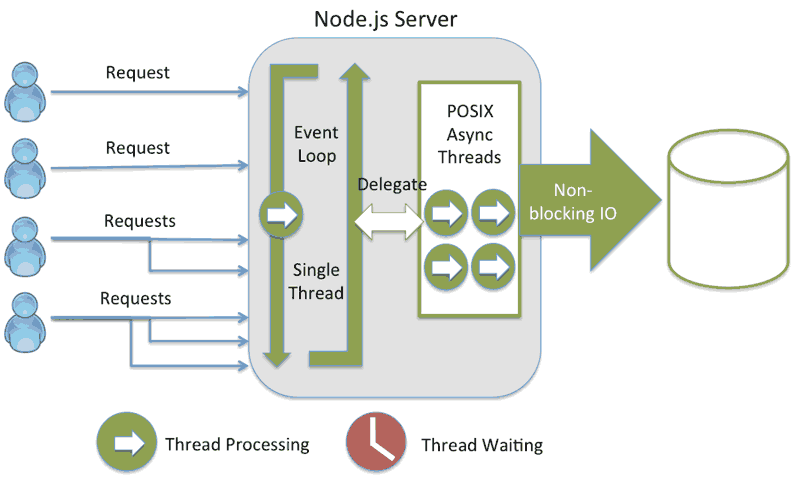
\includegraphics[width=0.9\textwidth]{img/node-js-structure.png}
    \caption{Struttura a single-thread di Node.js per la delegazione di thread asincroni in POSIX}
    \label{fig:async-node}
\end{figure}
 Sotto un punto di vista tecnico, vediamo che l'Event Loop viene gestito dal thread singolo della struttura di Node.js per andare ad inoltrare ogni richiesta ricevuta ad un thread asincrono POSIX che, per la sua natura, crea una procedura non bloccante per la gestione della request. In altre parole, il single thread serve solamente per la gestione degli inoltri di request e di response. 
\newpage
\subsection{Express.js}
Express.js è un framework basato su Node minimalista in grado di poter semplificare l'implementazione di alcune operazioni di base senza nessuna imposizione di vincoli. Questa caratteristica è stata alla base della diffusione di tale framework e dell'implementazione di librerie di terze parti capaci di poter gestire elementi di applicazioni web come cookie, parsing di richieste, gestione degli errori, del login e di gestione di componenti esterne comunicanti. Notiamo che un server in Node.js scritto in Express.js diventa più compatto:
\begin{lstlisting}
var express = require('express');  
var app = express();  
app.get('/', (req,resp)=> {  
  resp.send('Hello World');  
}).listen('8000');
\end{lstlisting}
Nell'esempio sopra riportato, possiamo vedere come si gestisce una richiesta su un URL di radice secondo un'approccio basato su REST in cui si ha la ricezione della request, e l'invio di un messaggio di una response da parte dell'applicazione Express in ascolto sulla porta 8000 in maniera asincrona.
\subsection{Architettura Docker}
Docker è un progetto open source nato con lo scopo di automatizzare la distribuzione di applicazioni sotto forma di contenitori leggeri, portabili e autosufficienti che possono essere eseguiti su cloud (pubblici o privati) o in locale. La tecnologia Docker si basa sul kernel di Linux che garantisce l'isolamento dei processi in modo tale da poter eseguirli in maniera indipendente. Tale caratteristica è alla base delle proprietà del container che riesce ad eseguire una applicazione andandone a rispettare tutte le dipendenze sfruttando l'infrastruttura esistente in modo da poter conservare un buon livello di sicurezza. 
I container Docker consentono il deployment a partire da un'immagine. Ciò semplifica la condivisione di un'applicazione o di un insieme di servizi, con tutte le loro dipendenze, nei vari ambienti. Un'altra caratteristica dei container di Docker è l'automatizzazione della distribuzione delle applicazioni o dei processi che la compongono attuando un meccanismo di replica basato sulla condivisione delle immagini dell'applicazione. Gli strumenti sviluppati partendo dai container Linux, responsabili dell'unicità e della semplicità di utilizzo di Docker, offrono agli utenti accesso alle applicazioni, la capacità di eseguire un deployment rapido, e il controllo sulla distribuzione di nuove versioni.
\begin{figure}[h]
    \centering
    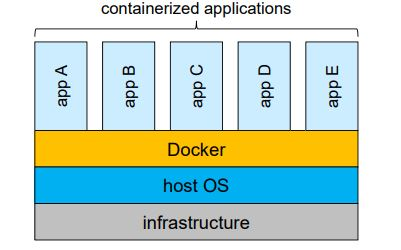
\includegraphics[width=0.9\textwidth]{img/infrastructure-docker.jpg}
    \caption{Struttura dell'architettura Docker}
    \label{fig:infrastructure-dockere}
\end{figure}
I vantaggi nell'utilizzo di Docker sono i seguenti: 
\begin{itemize}
    \item Modularità: la struttura dell'architettura si basa su vari container indipendenti in cui poter gestire varie applicazioni in maniera parallela e autosufficiente.
    \item Sistema di aggiornamento stratificato: Le immagini su cui si basano le applicazioni hanno una struttura stratificata. Ad ogni proprietà alterata dell'immagine, si crea un nuovo strato che andrà ad aggiungersi a quelli pre-esistenti.
    \item Meccanismo di rollback: uno dei maggiori vantaggi della stratificazione è la capacità di eseguire il rollback. Ogni immagine è composta da strati. Se l'iterazione di un'immagine non è soddisfacente, è possibile riportala alla versione precedente.
    \item Facilità di deploy: i container basati su Docker possono ridurre il deployment a pochi secondi. Creando un container per ogni processo, puoi condividere con rapidità i processi simili con le nuove applicazioni. Poiché non è necessario riavviare un sistema operativo per aggiungere o spostare un container, i tempi per il deployment sono sostanzialmente più brevi.
\end{itemize}

\newpage
